%%%%%%%%%%%%%%%%%%%%%%%%%%%%%%%%%%%%%%%%%
% Masters/Doctoral Thesis 
% LaTeX Template
% Version 2.1 (2/9/15)
%
% This template has been downloaded from:
% http://www.LaTeXTemplates.com
%
% Version 2.0 major modifications by:
% Vel (vel@latextemplates.com)
%
% Original authors:
% Steven Gunn  (http://users.ecs.soton.ac.uk/srg/softwaretools/document/templates/)
% Sunil Patel (http://www.sunilpatel.co.uk/thesis-template/)
%
% License:
% CC BY-NC-SA 3.0 (http://creativecommons.org/licenses/by-nc-sa/3.0/)
%
%%%%%%%%%%%%%%%%%%%%%%%%%%%%%%%%%%%%%%%%%

%----------------------------------------------------------------------------------------
%	PACKAGES AND OTHER DOCUMENT CONFIGURATIONS
%----------------------------------------------------------------------------------------

\documentclass[
11pt, % The default document font size, options: 10pt, 11pt, 12pt
%oneside, % Two side (alternating margins) for binding by default, uncomment to switch to one side
spanish, % ngerman for German
singlespacing, % Single line spacing, alternatives: onehalfspacing or doublespacing
%draft, % Uncomment to enable draft mode (no pictures, no links, overfull hboxes indicated)
%nolistspacing, % If the document is onehalfspacing or doublespacing, uncomment this to set spacing in lists to single
%liststotoc, % Uncomment to add the list of figures/tables/etc to the table of contents
%toctotoc, % Uncomment to add the main table of contents to the table of contents
%parskip, % Uncomment to add space between paragraphs
]{MastersDoctoralThesis} % The class file specifying the document structure

\usepackage[utf8]{inputenc} % Required for inputting international characters
\usepackage[T1]{fontenc} % Output font encoding for international characters

\usepackage{palatino} % Use the Palatino font by default

\usepackage[backend=bibtex,style=authoryear,natbib=true]{biblatex} % User the bibtex backend with the authoryear citation style (which resembles APA)

%\addbibresource{example.bib} % The filename of the bibliography

\usepackage[autostyle=true]{csquotes} % Required to generate language-dependent quotes in the bibliography

\usepackage{float}
\usepackage{graphicx}
\usepackage{caption}
%\usepackage{subfigure}


%----------------------------------------------------------------------------------------
%	THESIS INFORMATION
%----------------------------------------------------------------------------------------

\thesistitle{Ingeniería de descriptores para la detección automática de vasos sanguíneos en imágenes de fondo de ojo} % Your thesis title, this is used in the title and abstract, print it elsewhere with \ttitle
\supervisorfirst{Dra. Mariana \textsc{del Fresno}}
\supervisorsecond{Ing. José Ignacio \textsc{Orlando}}
% Your supervisor's name, this is used in the title page, print it elsewhere with \supname
\examiner{Nombres de los jurados} % Your examiner's name, this is not currently used anywhere in the template, print it elsewhere with \examname
\degree{Ingeniero de Sistemas} % Your degree name, this is used in the title page and abstract, print it elsewhere with \degreename
\author{\\Valeria \textsc{del Río} \\ Marcos \textsc{Fracchia} \\} % Your name, this is used in the title page and abstract, print it elsewhere with \authorname
\addresses{} % Your address, this is not currently used anywhere in the template, print it elsewhere with \addressname

\subject{Matemática Aplicada} % Your subject area, this is not currently used anywhere in the template, print it elsewhere with \subjectname
\keywords{} % Keywords for your thesis, this is not currently used anywhere in the template, print it elsewhere with \keywordnames
\university{{Universidad Nacional del Centro de la Provincia de Buenos Aires}} % Your university's name and URL, this is used in the title page and abstract, print it elsewhere with \univname
\department{Facultad de Ciencias Exactas} % Your department's name and URL, this is used in the title page and abstract, print it elsewhere with \deptname
\group{Facultad de Ciencias Exactas} % Your research group's name and URL, this is used in the title page, print it elsewhere with \groupname
\faculty{Universidad Nacional del Centro de la Provincia de Buenos Aires} % Your faculty's name and URL, this is used in the title page and abstract, print it elsewhere with \facname




\hypersetup{pdftitle=\ttitle} % Set the PDF's title to your title
\hypersetup{pdfauthor=\authorname} % Set the PDF's author to your name
\hypersetup{pdfkeywords=\keywordnames} % Set the PDF's keywords to your keywords

\begin{document}

\frontmatter % Use roman page numbering style (i, ii, iii, iv...) for the pre-content pages

\pagestyle{plain} % Default to the plain heading style until the thesis style is called for the body content

%----------------------------------------------------------------------------------------
%	TITLE PAGE
%----------------------------------------------------------------------------------------

\begin{titlepage}
\begin{center}

\textsc{\LARGE \univname}\\[1.5cm] % University name
\textsc{\Large Tesis de Grado}\\[0.5cm] % Thesis type

\HRule \\[0.4cm] % Horizontal line
{\huge \bfseries \ttitle}\\[0.4cm] % Thesis title
\HRule \\[1.5cm] % Horizontal line
 

\begin{centering} \large
\emph{Autores:}
\authorname
%\href{http://www.pladema.net/iorlando}{\authorname} \\ % Author name - remove the \href bracket to remove the link
\end{centering}
\vspace{0.6cm}
\begin{centering} \large
\emph{Directores:} \\
{\supnamef}\\ % Supervisor name - remove the \href bracket to remove the link  
{\supnames}\\ % Supervisor name - remove the \href bracket to remove the link  

\end{centering}
\vspace{0.6cm}

\large \textit{Trabajo de Tesis para optar al Título de \\ \degreename }\\[0.3cm] % University requirement text
\textit{de la}\\[0.4cm]
\deptname\\\facname\\[0.4cm] % Research group name and department name

{\large \today}\\[4cm] % Date
%\includegraphics{Logo} % University/department logo - uncomment to place it

\begin{centering} \large
\emph{Jurados:} \\
\examname \\
\end{centering}
\vspace{0.6cm}


 
\vfill
\end{center}
\end{titlepage}

%----------------------------------------------------------------------------------------
%	DECLARATION PAGE
%----------------------------------------------------------------------------------------



\cleardoublepage

%----------------------------------------------------------------------------------------
%	QUOTATION PAGE
%----------------------------------------------------------------------------------------

\vspace*{0.2\textheight}

\noindent\enquote{\itshape Thanks to my solid academic training, today I can write hundreds of words on virtually any topic without possessing a shred of information, which is how I got a good job in journalism.}\bigbreak

\hfill Dave Barry

%----------------------------------------------------------------------------------------
%	ABSTRACT PAGE
%----------------------------------------------------------------------------------------

\begin{abstract}
\addchaptertocentry{\abstractname} % Add the abstract to the table of contents

The Thesis Abstract is written here (and usually kept to just this page). The page is kept centered vertically so can expand into the blank space above the title too\ldots

\end{abstract}

%----------------------------------------------------------------------------------------
%	ACKNOWLEDGEMENTS
%----------------------------------------------------------------------------------------

\begin{acknowledgements}
\addchaptertocentry{\acknowledgementname} % Add the acknowledgements to the table of contents

The acknowledgements and the people to thank go here, don't forget to include your project advisor\ldots

\end{acknowledgements}

%----------------------------------------------------------------------------------------
%	LIST OF CONTENTS/FIGURES/TABLES PAGES
%----------------------------------------------------------------------------------------

\tableofcontents % Prints the main table of contents

\listoffigures % Prints the list of figures

\listoftables % Prints the list of tables




%----------------------------------------------------------------------------------------
%	DEDICATION
%----------------------------------------------------------------------------------------

\dedicatory{For/Dedicated to/To my\ldots} 

%----------------------------------------------------------------------------------------
%	THESIS CONTENT - CHAPTERS
%----------------------------------------------------------------------------------------

\mainmatter % Begin numeric (1,2,3...) page numbering

\pagestyle{thesis} % Return the page headers back to the "thesis" style

% Include the chapters of the thesis as separate files from the Chapters folder
% Uncomment the lines as you write the chapters

% Chapter 1

\chapter{Introducci\'on} % Main chapter title

\label{Chapter1} % For referencing the chapter elsewhere, use \ref{Chapter1} 

%----------------------------------------------------------------------------------------

% Define some commands to keep the formatting separated from the content 
\newcommand{\keyword}[1]{\textbf{#1}}
\newcommand{\tabhead}[1]{\textbf{#1}}
\newcommand{\code}[1]{\texttt{#1}}
\newcommand{\file}[1]{\texttt{\bfseries#1}}
\newcommand{\option}[1]{\texttt{\itshape#1}}

%----------------------------------------------------------------------------------------

\section{Welcome and Thank You}


%----------------------------------------------------------------------------------------

\section{Learning \LaTeX{}}


\subsection{A (not so short) Introduction to \LaTeX{}}

\subsection{A Short Math Guide for \LaTeX{}}


\subsection{Common \LaTeX{} Math Symbols}

\subsection{\LaTeX{} on a Mac}
 

%----------------------------------------------------------------------------------------

\section{Getting Started with this Template}



\subsection{About this Template}



%----------------------------------------------------------------------------------------

\section{What this Template Includes}

\subsection{Folders}



\subsection{Files}


%----------------------------------------------------------------------------------------

\section{Filling in Your Information in the \file{main.tex} File}\label{FillingFile}


%----------------------------------------------------------------------------------------

\section{The \code{main.tex} File Explained}


%----------------------------------------------------------------------------------------

\section{Thesis Features and Conventions}\label{ThesisConventions}


\subsection{Printing Format}


\subsection{Using US Letter Paper}



\subsection{References}


\subsection{Tables}

Tables are an important way of displaying your results, below is an example table which was generated with this code:

{\small
\begin{verbatim}
\begin{table}
\caption{The effects of treatments X and Y on the four groups studied.}
\label{tab:treatments}
\centering
\begin{tabular}{l l l}
\toprule
\tabhead{Groups} & \tabhead{Treatment X} & \tabhead{Treatment Y} \\
\midrule
1 & 0.2 & 0.8\\
2 & 0.17 & 0.7\\
3 & 0.24 & 0.75\\
4 & 0.68 & 0.3\\
\bottomrule\\
\end{tabular}
\end{table}
\end{verbatim}
}

\begin{table}
\caption{The effects of treatments X and Y on the four groups studied.}
\label{tab:treatments}
\centering
\begin{tabular}{l l l}
\toprule
\tabhead{Groups} & \tabhead{Treatment X} & \tabhead{Treatment Y} \\
\midrule
1 & 0.2 & 0.8\\
2 & 0.17 & 0.7\\
3 & 0.24 & 0.75\\
4 & 0.68 & 0.3\\
\bottomrule\\
\end{tabular}
\end{table}

You can reference tables with \verb|\ref{<label>}| where the label is defined within the table environment. See \file{Chapter1.tex} for an example of the label and citation (e.g. Table~\ref{tab:treatments}).

\subsection{Figures}

There will hopefully be many figures in your thesis (that should be placed in the \emph{Figures} folder). The way to insert figures into your thesis is to use a code template like this:
\begin{verbatim}
\begin{figure}
\centering

\includegraphics{Figures/Electron}
\decoRule
\caption[An Electron]{An electron (artist's impression).}
\label{fig:Electron}
\end{figure}
\end{verbatim}
Also look in the source file. Putting this code into the source file produces the picture of the electron that you can see in the figure below.

\begin{figure}[h]
\centering

\includegraphics{Figures/Electron}
\decoRule
\caption[An Electron]{An electron (artist's impression).}
\label{fig:Electron}
\end{figure}



\subsection{Typesetting mathematics}


You can write an equation, which is automatically given an equation number by \LaTeX{} like this:
\begin{verbatim}
\begin{equation}
E = mc^{2}
\label{eqn:Einstein}
\end{equation}
\end{verbatim}

This will produce Einstein's famous energy-matter equivalence equation:
\begin{equation}
E = mc^{2}
\label{eqn:Einstein}
\end{equation}

All equations you write (which are not in the middle of paragraph text) are automatically given equation numbers by \LaTeX{}. If you don't want a particular equation numbered, use the unnumbered form:
\begin{verbatim}
\[ a^{2}=4 \]
\end{verbatim}

%----------------------------------------------------------------------------------------

\section{Sectioning and Subsectioning}



%----------------------------------------------------------------------------------------

\section{In Closing}


% Chapter Template
%\usepackage{subfig}
\chapter{Estado del Arte} % Main chapter title

\label{Chapter2} % Change X to a consecutive number; for referencing this chapter elsewhere, use \ref{ChapterX}

%----------------------------------------------------------------------------------------
%	SECTION 1
%----------------------------------------------------------------------------------------

\section{An\'alisis de im\'agenes de la retina}

El an\'alisis de im\'agenes de la retina es de gran importancia para la detecci\'on de enfermedades del ojo.
El avance tecnol\'ogico permiti\'o obtener im\'agenes de la retina de mayor calidad, lo que beneficia que el analisis de estas permita la detecci\'on precoz de enfermedades con mayor precisi\'on, favoreciendo la disminuci\'on del porcentaje de personas con ceguera debido a enfermedades sistemicas o retinales. 

(---)
Existen muchas ventajas en el uso del an\'alisis de imagen digital para cuantificar la extensi\'on de la patolog\'ia de la retina en enfermedades vasculares, retinopat\'ia diab\'etica, degeneraci\'on macular asociada a la edad, y otras condiciones. Los beneficios clave incluyen la accesibilidad inmediata, visualizaci\'on, sistemas de gesti\'on de im\'agenes que permiten el seguimiento de la progresi\'on de la enfermedad mediante la revisi\'on de im\'agenes secuenciales, y la educaci\'on del paciente. Al mismo tiempo las im\'agenes capturadas, tienen una  gran resoluci\'on y se pueden visualizar en una pantalla tan pronto como se obtienen, y  permitiendo detectar y corregir cualquier error en el proceso fotogr\'afico a la vez.
(Lo anterior referencia a -Imaging the Retina  José Cunha- Vaz)

%-----------------------------------
%	SUBSECTION 1
%-----------------------------------
\subsection{Introducci\'on}

La retina es un tejido en capas que recubre el interior del ojo, permitiendo la conversión de la luz entrante en señales neuronales adecuadas para su posterior procesamiento por parte de la corteza visual del cerebro. La misma está sostenida por el epitelio pigmentario retinal, la coroide y la esclera.
La estructura anatómica del ojo se compone básicamente por la córnea (transparente), la esclera (normalmente blanca), el iris (que da color al ojo) y la pupila. Todas estas partes son visibles desde el exterior, y son las responsables de permitir la visión: un rayo de luz pasa a través de la córnea, que enfoca parcialmente la imagen, luego pasa por la cámara anterior, la pupila (que hace las veces de lente y enfoca aún más la imagen), la vítrea y por último es enfocado en la retina.

\begin{figure}[H]
	{
	\centering
	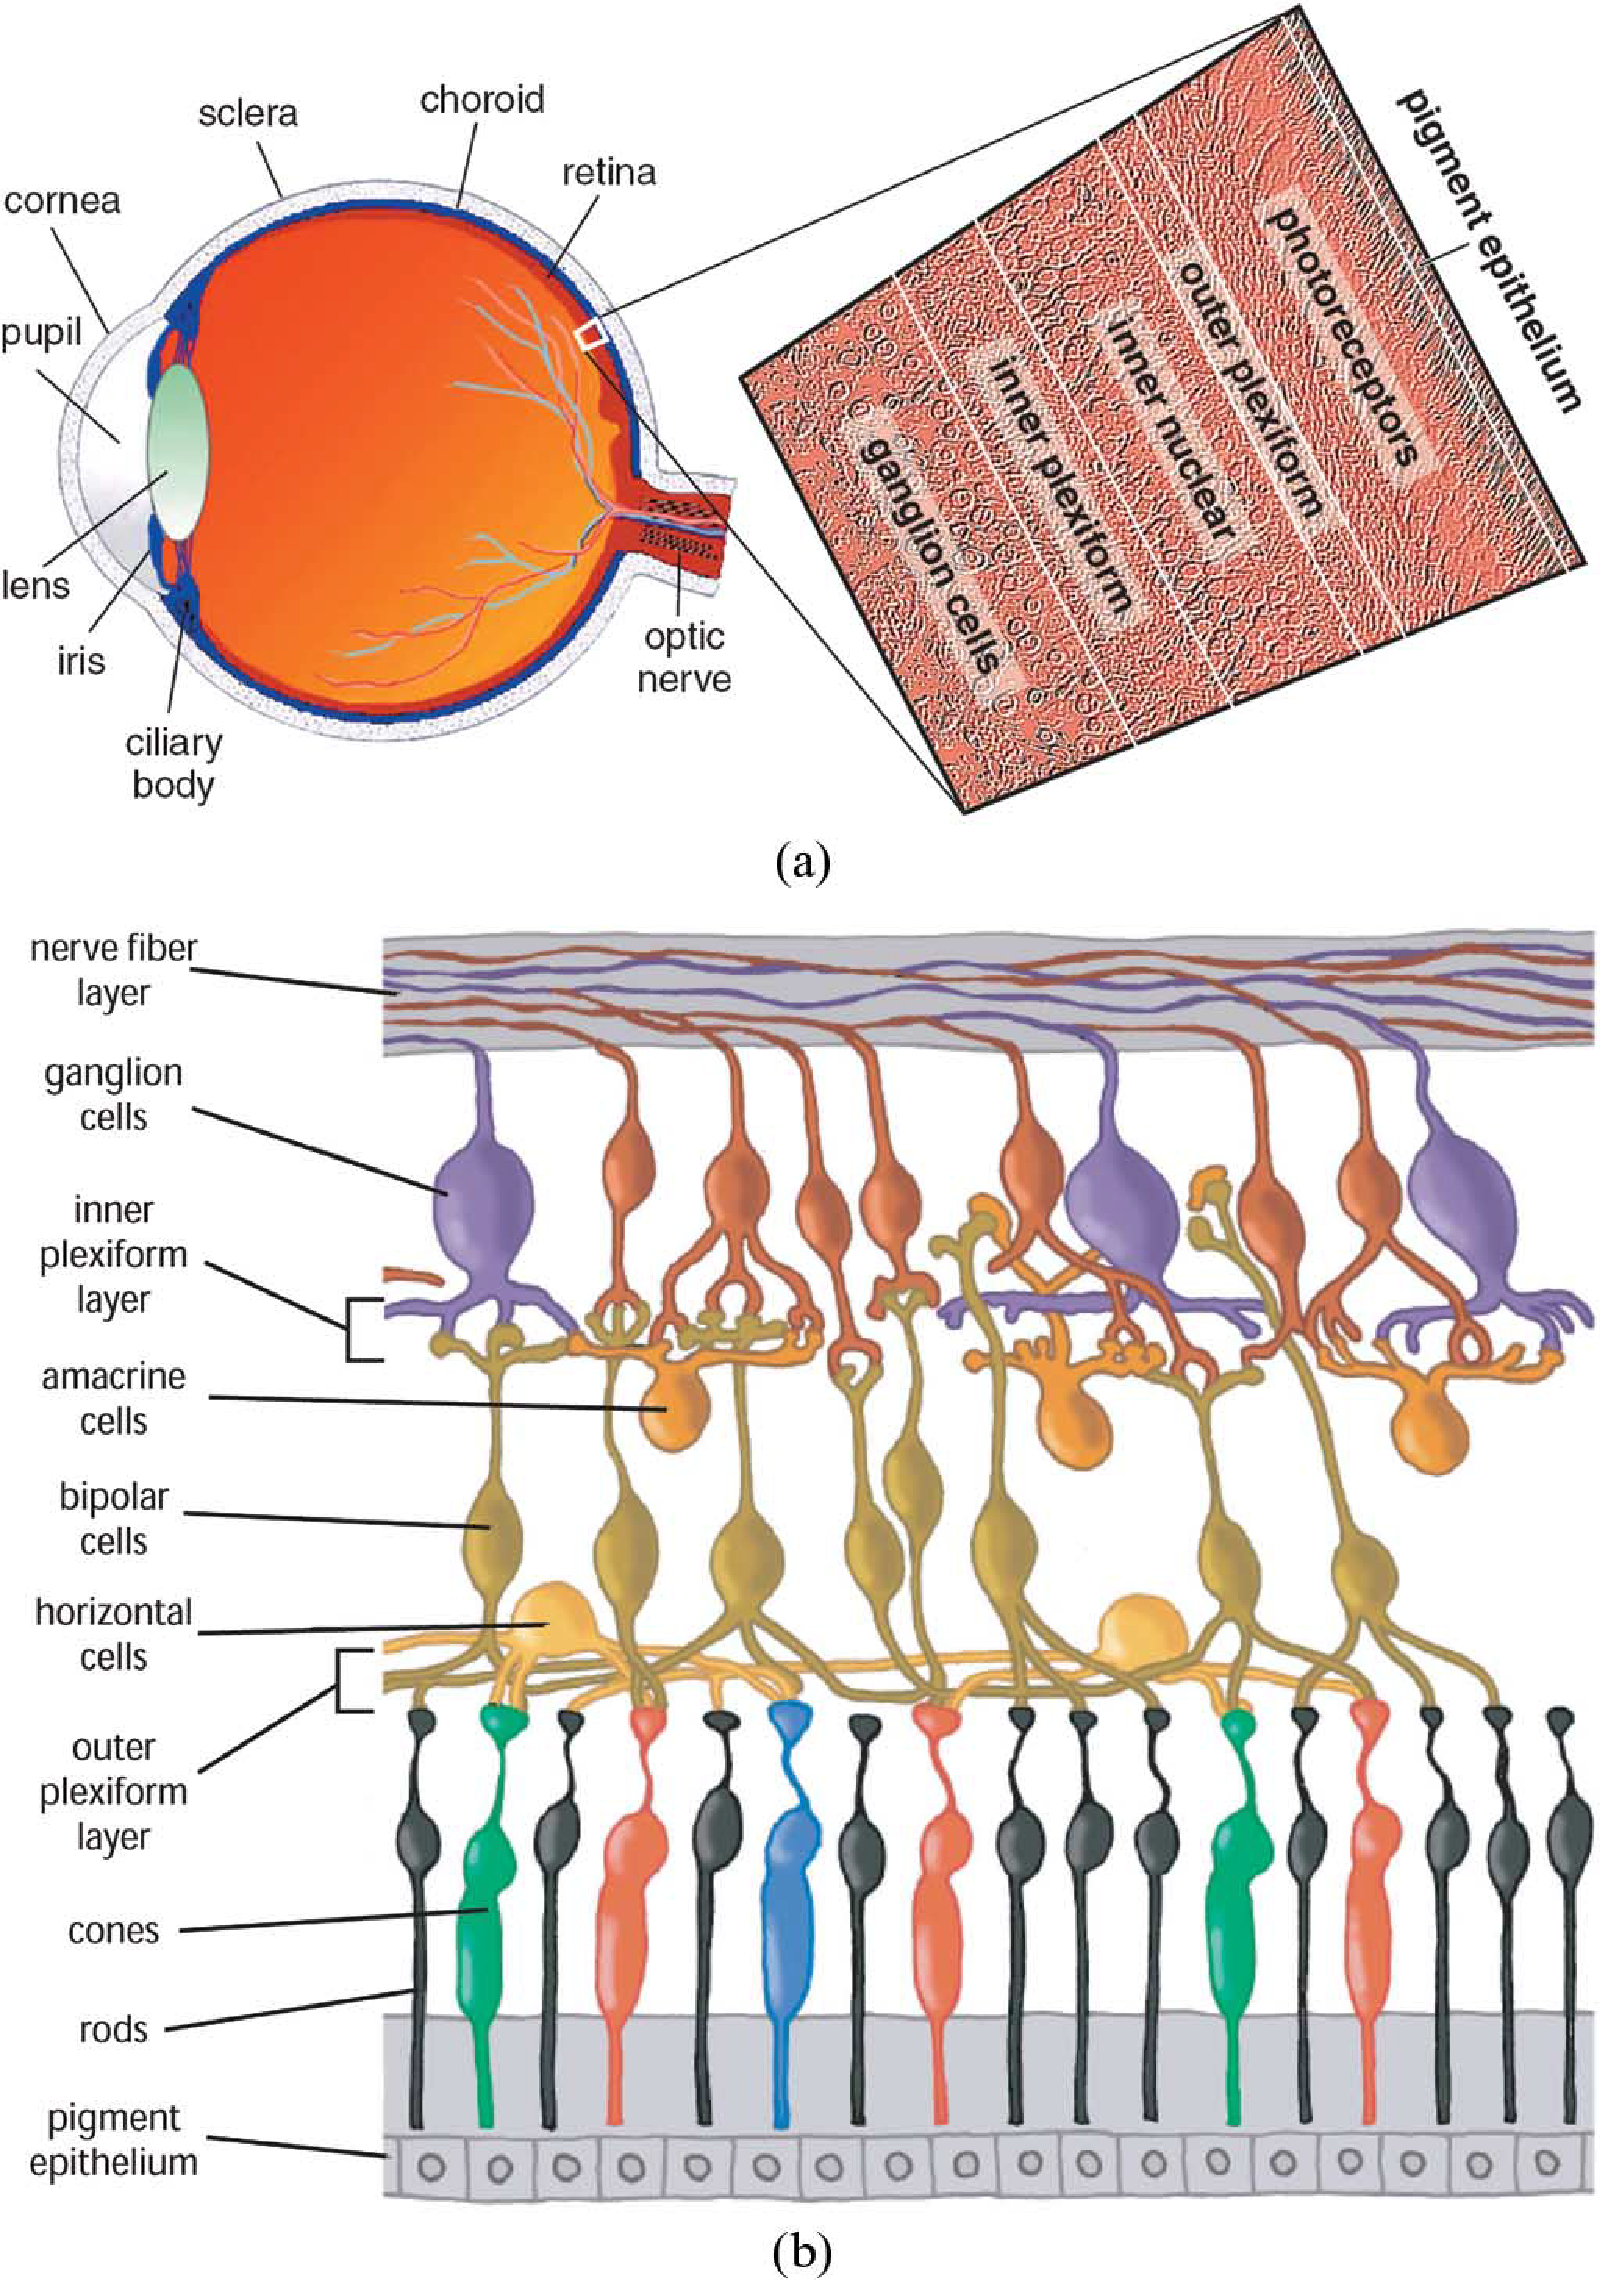
\includegraphics[width=0.75\textwidth]{Figures/ojo}
	\caption[Anatom\'ia del ojo 0-200]{\'Anatom\'ia del ojo. Ilustraci\'in de la anatom\'ia del ojo y capas de la retina [2], [3]. (A) Vista transversal del ojo y sus estructuras principales. La retina es un tejido delgado transparente que recubre la parte posterior del ojo y se compone de un n\'umero de capas, como se ilustra en la parte ampliada. (B) Representaci\'on esquem\'atica de las capas celulares de la retina. (a) Ilustraci\'on bidimensional de la anatom\'ia del ojo. (b)Representaci\'on esquem\'atica de las capas de la retina. Ejemplos de Kolb [3] utilizado con el permiso de Sigma Xi, The Scientific Sociedad de Investigación, Research Triangle Park, Carolina del Norte.}
	\label{fig:AnatomiaDelOjo}
	}
\end{figure}	

Durante la \'ultima d\'ecada, la fotograf\'ia digital a color ha sido reconocida como una modalidad aceptable para documentar el aspecto de la retina, ya que proporciona informaci\'on vital sobre la salud del paciente de la parte sensorial del sistema visual. La segmentaci\'on y el an\'alisis de im\'agenes de la retina se pueden utilizar para detectar el riesgo patol\'ogico o da\~nos, y asistir en el diagn\'ostico. 

El avance en la tecnologia aplicada en las imagenes digitales y  el aumento de la potencia de c\'alculo en dispositivos de procesamiento digital, presentan la posibilidad de utilizar estas tecnolog\'ias en oftalmolog\'ia. La microvasculatura retinal es \'unica, ya que es la \'unica parte de la circulaci\'on humana que puede ser visualizada directamente de forma no invasiva in vivo, fotografiando f\'acilmente el ojo, permitiendo el an\'alisis de las im\'agenes digitales.
(Lo anterior referencia a -> Retinal image analysis: Concepts,applications and potential)

T\'ecnicas de procesamiento de imágenes, análisis y visión a traves de dispositivos computacionales se encuentran hoy en d\'ia en todos los campos de la ciencia m\'edica. Estas técnicas son especialmente relevantes para la oftalmología moderna, un campo que depende en gran medida de los datos visuales. Las im\'agenes de la retina son ampliamente utilizadas por ofatalm\'ologos para fines de diagn\'ostico. Sin embargo, estas im\'agenes a menudo necesitan mejoras visuales antes de determinar un an\'alisis digital de riesgo patol\'ogico o la detecci\'on de da\~nos. 
(Lo anterior referencia a -> Marrugo2011)

(---)
En el modo tradicional de diagn\'ostico, los oftalm\'ologos examinan las im\'agenes de la retina, buscan las posibles anomal\'ias y entregan un diagn\'ostico. El procesamiento y ana\'lisis de la retina autom\'atico permite ahorrar carga de trabajo y puede ayudar a lograr una detecci\'on mas objetiva a los oftalm\'ologos. Se han hecho esfuerzos para extraer estructuras normales y anormales en im\'agenes de la retina de forma autom\'atica y robusta. La aplicaci\'on de t\'ecnicas de procesamiento de im\'agenes por computadora, para el an\'alisis de las im\'agenes de la retina comenz\'o aproximadamente hacia 1974 [1]. Desde entonces, mucho investigadores han presentado inter\'es en el tema, y han tenido que afrontar diversas dificultades, principalmente los ruidos, iluminaci\'on desigual y la variaci\'on entre los individuos. 
(Lo anterior referencia a -> li2004)

Las enfermedades que pueden manifestarse en el ojo pueden ser b\'asicamente de dos tipos, del ojo en s\'i mismo o sist\'emicas. Existen un conjunto de las mismas que pueden ser detectadas a trav\'es de la captura y el an\'alisis de im\'agenes de distintas estructuras de la retina. Las mismas pueden ser originadas, ya sea, en el ojo mismo, en el cerebro o en el sistema cardiovascular.
Dentro de las enfermedades que pueden diagnosticarse a trav\'es del an\'alisis de im\'agenes de la retina, se encuentra la retinopat\'ia diab\'etica (DR), una complicaci\'on de la Diabetes Mellitus, que afecta a un tercio de los diab\'eticos  y es la principal causa de p\'erdida de visi\'on en personas de edad avanzada,  y sigue siendo una de las principales causas de ceguera evitable. El edema macular diab\'etico (DME), caracterizado por el aumento de la permeabilidad vascular y la deposici\'on de exudados duros en la retina central, puede desarrollarse en cualquier etapa de la DR y aflige a 21 millones de personas en el mundo.  A trav\'es de ex\'amenes peri\'odicos de la vista, la p\'erdida de la visi\'on relacionada con la diabetes se puede prevenir en el 98\% de los casos.
(Lo anterior referencia a -> g0h2016)
Otra de las enfermedades diagnosticable mediante el an\'alisis de im\'agenes ret\'inales es la degeneraci\'on macular asociada a la edad (DMAE), la cual es la causa mas frecuente de ceguera en pa\'ises desarrollados en personas mayores de 50 anos. Una de las principales medidas para definir la gravedad de la DMAE, es el an\'alisis de derrames, alteraciones pigmentarias, atrofia geogr\'afica  y neovascularizaci\'on coroidea a partir de la proyecci\'on de im\'agenes de fondo de ojo, la tomograf\'ia de coherencia \'optica (OCT) y otras modalidades. Cada una de estas modalidades de imagen tienen puntos fuertes y puntos d\'ebiles para detectar, capturar y / o cuantificar diferentes patolog\'ias. Los tratamientos actuales para la DMAE no pueden curar o revertir la p\'erdida de la visi\'on. Sin embargo, el estudio de las enfermedades oculares relacionadas con la edad, mostr\'o que la suplementaci\'on con vitamina antioxidante espec\'ifica reduce el riesgo de progresi\'on de etapas intermedias, siendo una estrategia preventiva en pacientes correctamente identificados. De este modo la identificaci\'on temprana de pacientes con DMAE es importante para diseñar e implementar estrategias preventivas para el tratamiento del DMAE, y determinar su relaci\'on coste-eficacia. Mediante la teleoftalmolog\'ia o la telemedicina en combinaci\'on con la asistencia de una computadora o dispositivo, se puede realizar el an\'alisis de comunidades alejadas de zonas urbanas o situadas en zonas de riesgo, permitiendo identificar a individuos que padezcan alguna patolog\'ia retinal, en una etapa temprana, a modo de prevenci\'on.
(Lo anterior referencia a ->Progress on retinal image analysis for age related macular degeneration )

Actualmente existen diversas \'areas de investigación activas en lo que respecta a la imagenología de la retina. Algunas de las \'areas se centran en la b\'usqueda de herramientas rentables, f\'aciles de usar y portables, que asistan en el análisis y procesamiento de las imágenes. Por otro lado CONSULTAR IMAGENES FUNCIONALES. Adaptive Optics o \'optica adaptativa, es otra \'area que se encarga de la utilizaci\'on de lentes para corregir las fallas de frente de onda de la luz reflejada desde la retina, permitiendo la obtenci\'on de celulas individuales o estructuras celulares.
Longer Wavelength OCT Imaging o longitud de onda m\'as larga, realiza investigaciones para el desarrollo de los l\'aseres de baja coherencia de c\'odigo de barrido con longitudes de ondas centrales mayores. Algunos de estos prototipos ya son capaces de resolver los detalles en la coroides y la l\'amina cribosa.

%-----------------------------------
%	SUBSECTION 2
%-----------------------------------

\subsection{Fotograf\'ias de fondo de ojo}

Existen diversas formas de poder observar y analizar la anatom\'ia del ojo, a trav\'es de im\'agenes m\'edicas. 
Una de las modalidades de imagen m\'edica que permite explorar el interior del ojo es la de la imagen de fondo de ojo. La misma consiste en  una representaci\'on 2D del tejido retinal semitransparente 3D, proyectado en el plano de obtenci\'on de la imagen, que se obtiene usando la luz reflejada en el tejido.
Para realizar la captura del fondo de ojo, se dilata la pupila con f\'armacos que se depositan en forma de gotas en la superficie ocular; as\'i, el oftalm\'ologo puede ver con facilidad el interior del globo ocular con un aparato que se llama oftalmoscopio. El oftalmoscopio consiste en un aparato formado por una serie de espejos y cristales que alumbran la retina del ojo sin que la luz se refleje. Si no fuese por el oftalmoscopio la luz provocar\'ia destellos y no se podría ver el fondo de ojo de manera correcta, algo parecido a lo que sucede cuando el flash de una cámara de fotos saca los ojos en color rojo. Esta modalidad no es invasiva, y su costo es menor a la angiografía y la OCT dado que la c\'amara que se necesita para capturar la imagen del ojo es una c\'amara digital convencional.
Adem\'as de facilitar la detecci\'on de enfermedades oculares, las im\'agenes de fondo de ojo permiten detectar tres tipos de lesiones oculares. 

La exploraci\'on del fondo de ojo se realiza para visualizar a trav\'es de la pupila la porci\'on posterior e interior del ojo. Gracias a este procedimiento pueden observarse diferentes estructuras internas del globo ocular: m\'acula, retina y papila \'optica entre otras. Tambi\'en es posible visualizar directamente los vasos sangu\'ineos de la retina.
(wiki)
Para realizar la captura, se utiliza una c\'amara digital encargada de tomar la im\'agen del interior del ojo. Se utiliza un oftalmoscopio de baja potencia que se conecta con la c\'amara digital, este diseño realiza la captura de la fotograf\'ia del fondo del ojo y utiliza la luz del espectro visible para obtener im\'agenes de la estructura de la retina in vivo. En im\'agenes en color, las intensidades de imagen representan la cantidad de longitudes de ondas rojas, verdes y azules reflejadas, como se determina por la sensibilidad espectral del sensor. Dado que el nivel de luz ambiental crea insuficiente iluminaci\'on reflejada por la imagen digital, la iluminaci\'on interior debe ser proyectada en el ojo, y la luz reflejada por la retina debe volver al plano pupilar. Es decir, que se debe proyectar un haz de luz (flash) sobre el ojo, para iluminar el \'organo ocular y obtener una mejor imagen del fondo del ojo.
(Lo anterior referencia a -> Progress on retinal image analysis for age related macular degeneration)


\begin{figure}
\centering
\begin {subfigure}
	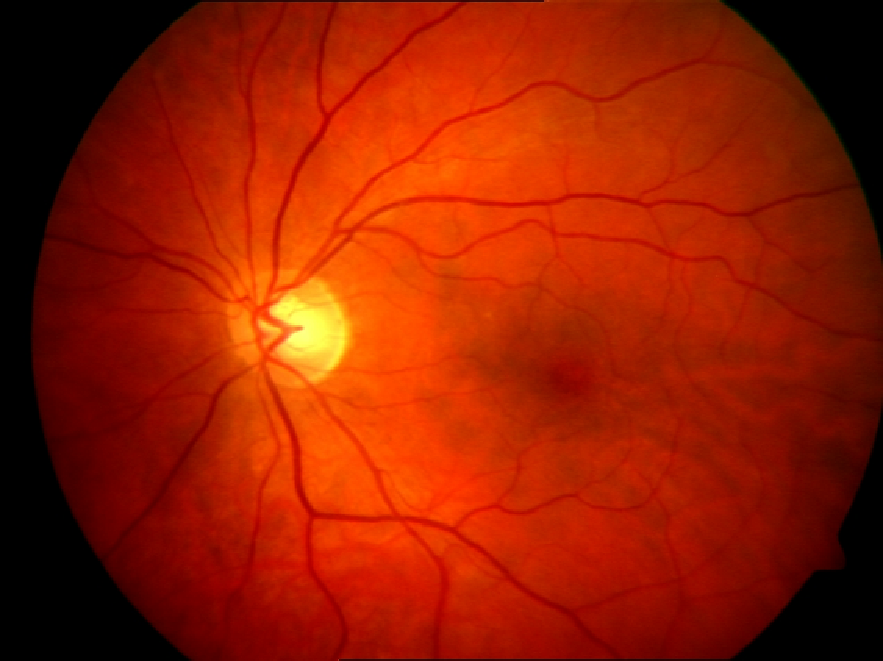
\includegraphics[width=23mm]{Figures/images}
	\caption{Dataset ARIA}
\end{subfigure}
\quad
\begin {subfigure}
	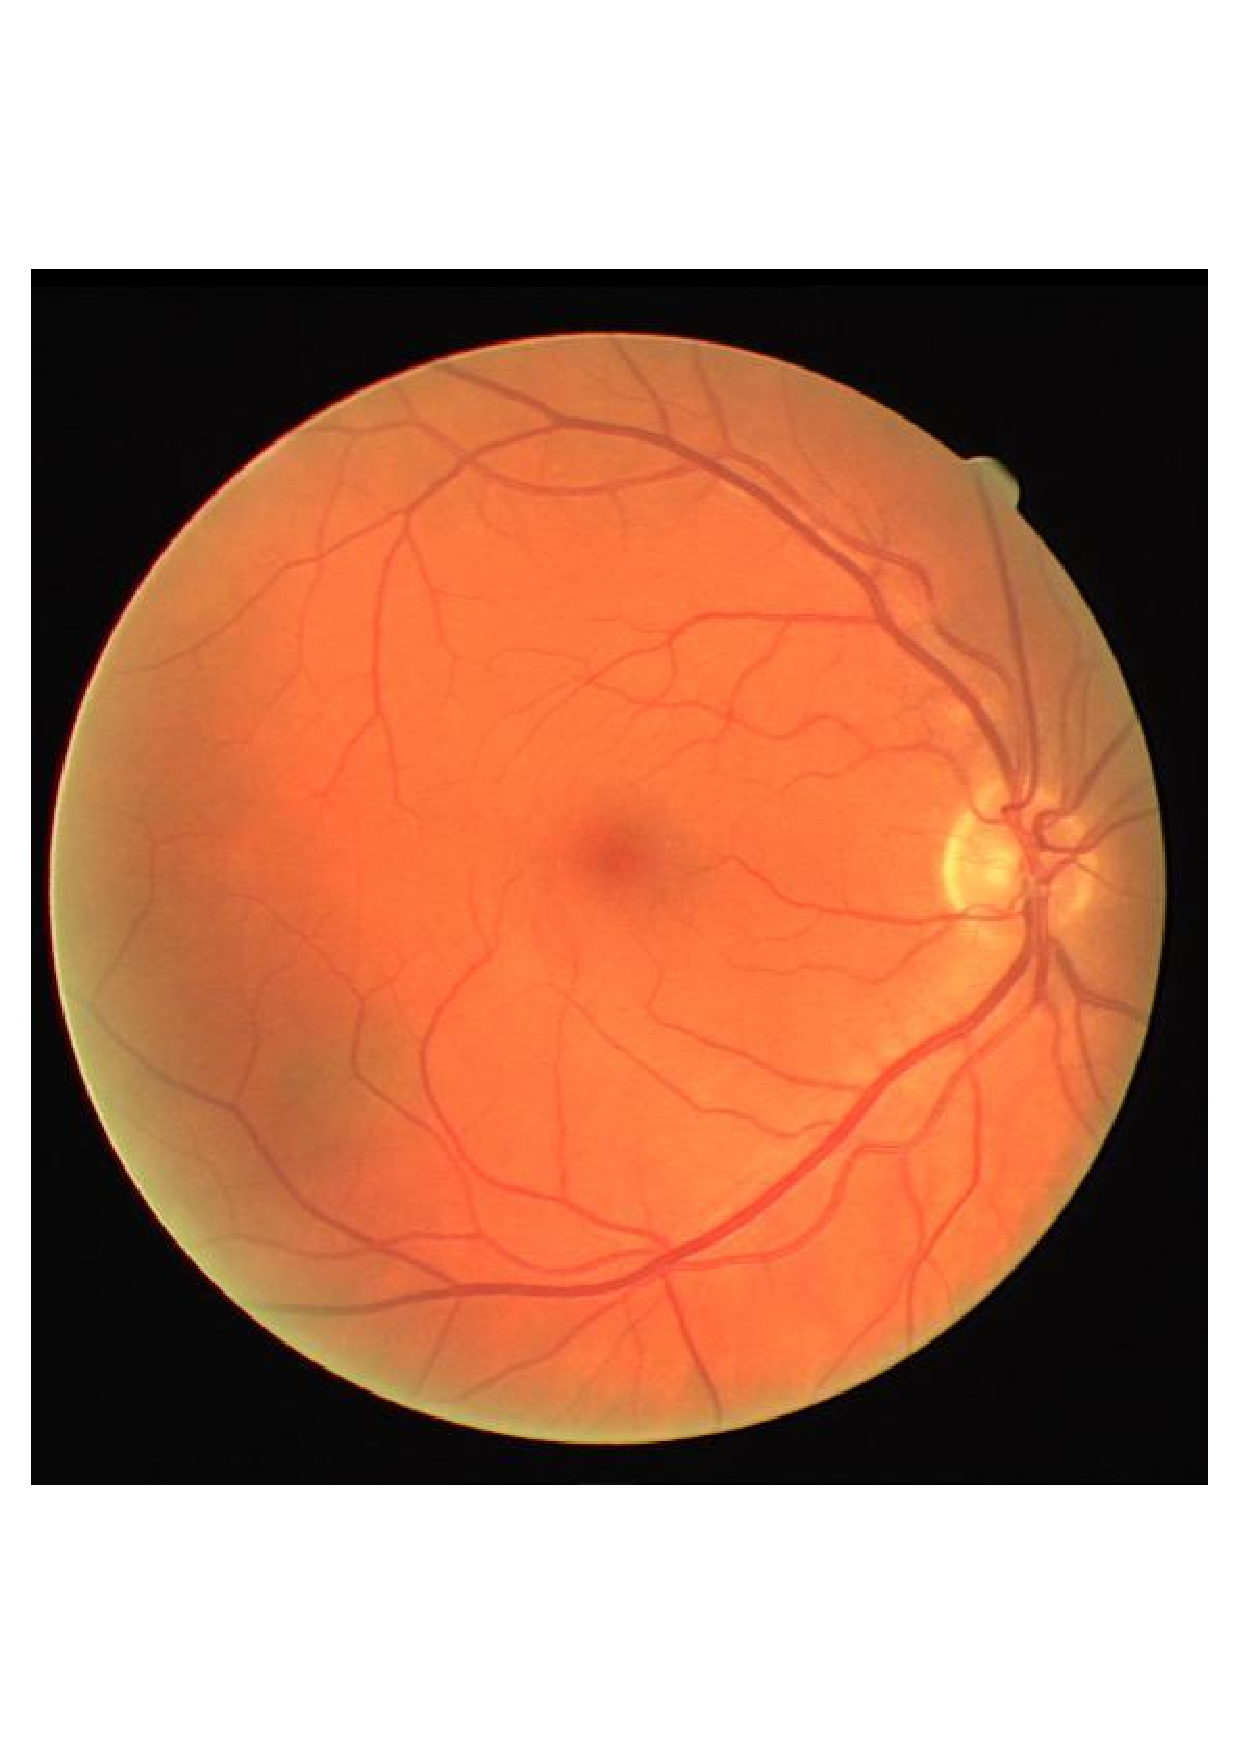
\includegraphics[width=23mm]{Figures/images1}
	\caption{Dataset HRF}
\end{subfigure}
\quad
\begin {subfigure}
	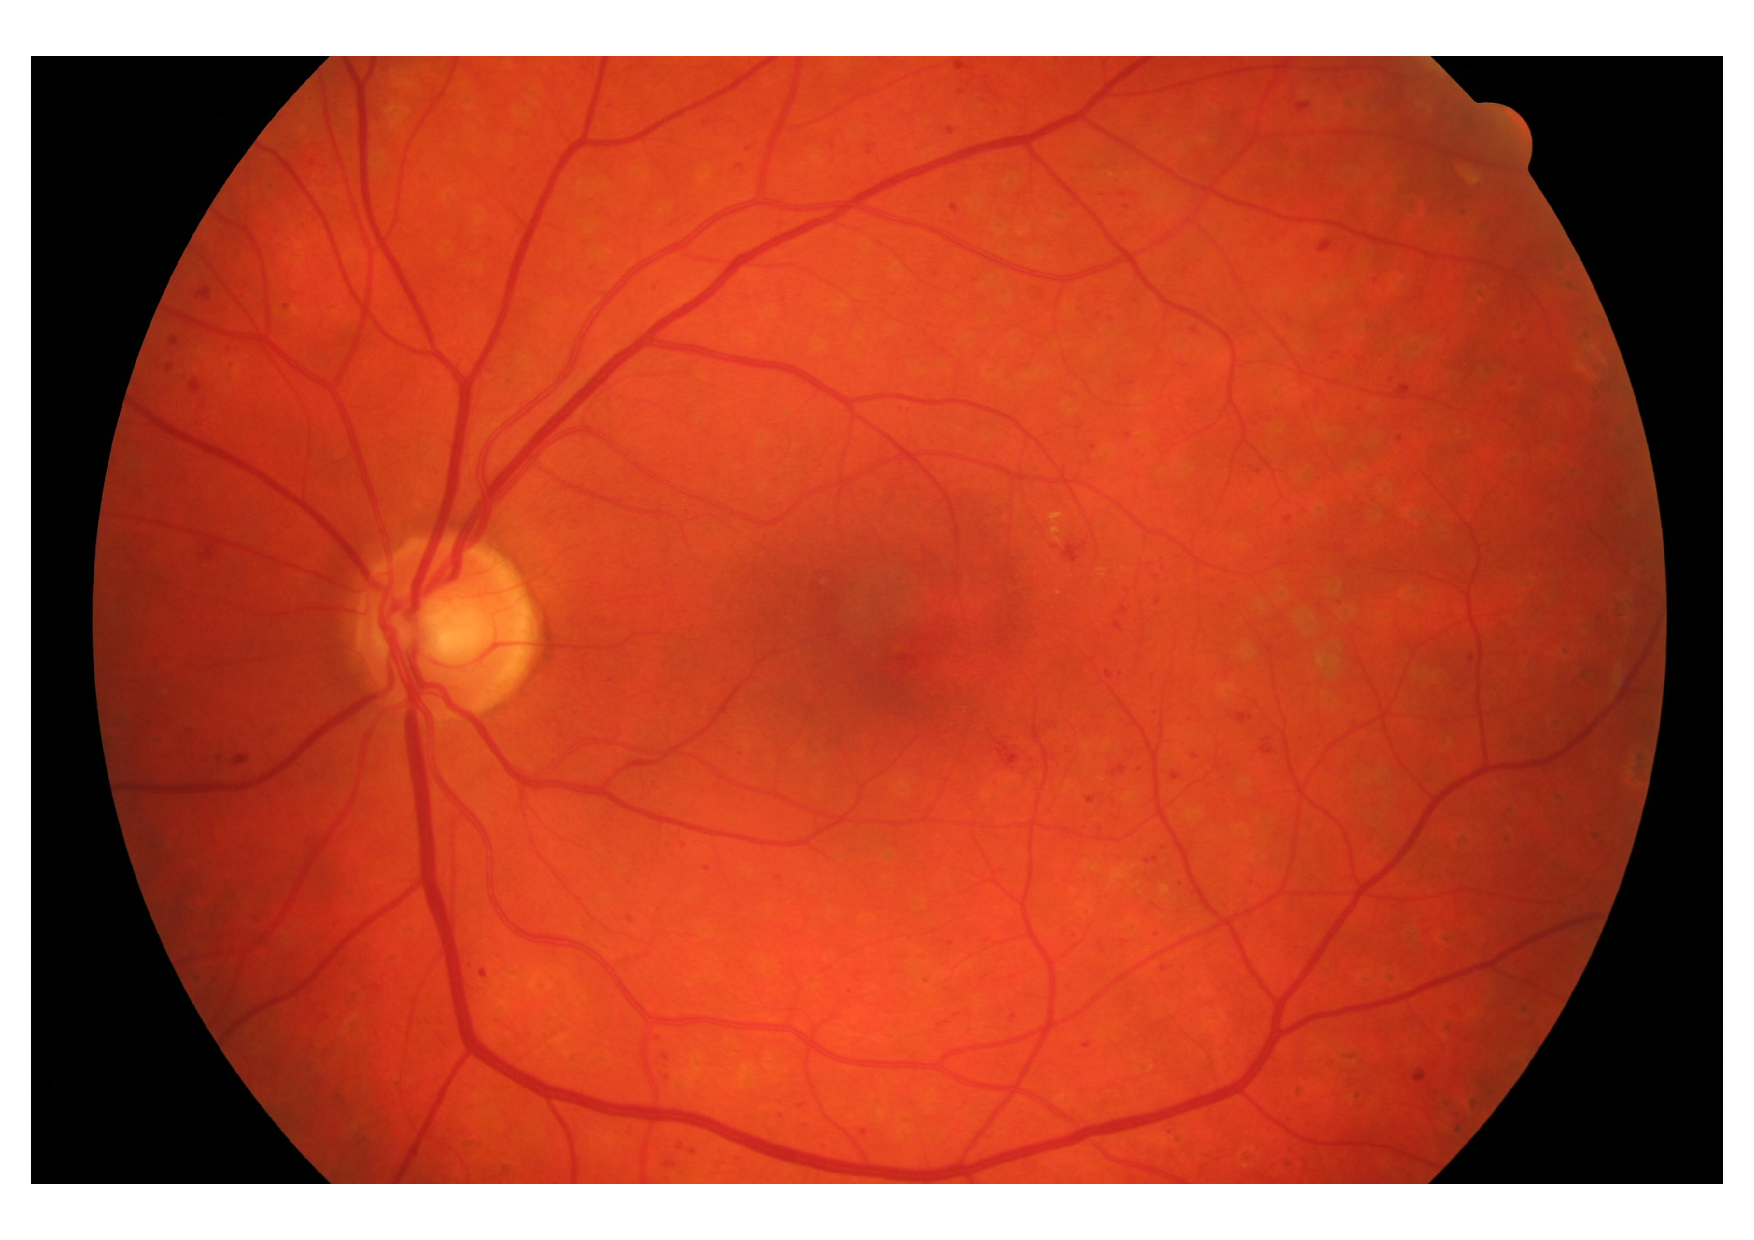
\includegraphics[width=23mm]{Figures/images2}
	\caption{Dataset DRIVE}
\end{subfigure}
\end{figure}

El Instituto Nacional del Reino Unido (NICE) establece que una prueba de cribado de RD debe tener la sensibilidad y la especificidad de al menos el 80\% y 95\%, respectivamente, con una tasa de fallo t\'ecnico inferior al 5\%. El m\'etodo de la fotograf\'ia est\'andar para la detecci\'on de DR es la fotograf\'ia en color de fondo de ojo estereosc\'opica en 7 campos (30$^{\circ}$) definidas por el grupo de tratamiento temprano de la retinopat\'ia diab\'etica Study (ETDRS). También es \'util para la identificaci\'on de DME y la neovascularizaci\'on retinal sutil. Sin embargo, desde la perspectiva del paciente, teniendo 7 campos es mucho tiempo, tediosa e inc\'omoda.
Actualmente se utilizan  2 o 3 campos para el cribado en la fotograf\'ia de fondo de ojo, ya que representan un compromiso razonable de la sensibilidad y buena  comodidad para el paciente.
La fotograf\'ia de fondo midr\'iatico ha demostrado ser una estrat\'egia eficaz de cribado de DR. Ofrece una sensibilidad de al menos 80\% en la detecci\'on de cualquier grado de DR, y la sensibilidad y especificidad de 97\% y 92\%, respectivament.
El uso de sistemas de im\'agenes digitales ha reducido la tasa de fallo t\'ecnico asociado con la fotograf\'ia de pel\'icula anterior no digital, y la imagen electr\'onica que permite un f\'acil almacenamiento y catalogaci\'on. Los sistemas digitales modernos utilizados en la fotograf\'ia de fondo de ojo han demostrado lograr una sensibilidad y especificidad de aproximadamente el 90\% en la detecci\'on de DR.
Lo anterior referencia a -> g0h2016


%-----------------------------------
%	SUBSECTION 3
%-----------------------------------

\subsection{Herramientas computacionales para an\'alisis de fotograf\'ias de fondo de ojo}
En la actualidad para realizar el an\'alisis de un  estudio de fondo de ojo, se puede recurrir a la tecnolog\'ia, ya que la complejidad y la sobrecarga que puede sufrir el profesional pueden hacer de la tarea de an\'alisis algo complejo o imposible. Actualmente existe un gran volumen de informaci\'on generada por los distintos dispositivos de captura, y para lograr manipularlo podemos recurrir a la utilizaci\'on de distintas t\'ecnicas avanzadas de procesamiento, an\'alisis y visualizaci\'an de im\'agenes, como as\'i tambi\'en a la construcci\'on de modelos computacionales y de simulaci\'on.
Dentro de las etapas del procesamiento de im\'agenes, un primer grupo de algoritmos se asocian con el pre-procesamiento y realce. Esta etapa puede resultar particularmente importante a fin de reducir el ruido o distorsiones que pueden afectar la informaci\'on presente en las im\'agenes, o para la extracci\'on de caracter\'isticas de inter\'es, seg\'un la aplicaci\'on en particular. Otro proceso importante es la segmentaci\'on, que permite la detecci\'on de diferentes estructuras dentro de la imagen y la construcci\'on de modelos geom\'etricos asociados, para su an\'alisis y visualizaci\'on, o sobre los cuales realizar la planificaci\'on y simulaci\'on de tratamientos. A partir de la informaci\'on obtenida de la imagen, por medio de estrategias de an\'alisis es posible reconocer patrones o extraer diferentes indicadores cuantitativos para evaluar la extensi\'on o distribuci\'on de una determinada estructura o patolog\'ia.
Entre otras aplicaciones, con este tipo de procesamientos se puede detectar, por ejemplo, una patolog\'ia en una imagen de fondo de ojo y analizar su variaci\'on en diferentes estadios de un tratamiento. Tambi\'en es posible extraer el \'arbol vascular o evidenciar estructuras patol\'ogicas y as\'i asistir en el diagn\'ostico y tratamiento de enfermedades, como la retinopat\'ia diab\'etica que puede provocar la reducci\'on o p\'erdida de la capacidad visual. Tambi\'en es factible la contribuci\'on al desarrollo de modelos personalizados de simulaci\'on para el estudio de enfermedades y su tratamiento.
 Esta digitalizaci\'on de los estudios y datos m\'edicos, conlleva al uso de sistemas de archivo y comunicaci\'on de im\'agenes conocidos como PACS (por Picture Archiving and Communication System), para la gesti\'on eficiente de las im\'agenes m\'edicas. Estos sistemas deben cumplir con el est\'andar DICOM (Digital Imaging and Communication of Medical Imaging) para su transmisi\'on y almacenamiento y con el est\'andar HL-7 (Health Level 7) para la transmisi\'on de datos m\'edicos, permitiendo la interconectividad de los equipos y terminales de trabajo, bajo determinados protocolos de seguridad.
Los aspectos más importantes en esta \'area se asocian a las telecomunicaciones, la inform\'atica m\'edica y los servicios de salud. Por medio de estos sistemas y est\'andares no solo es posible la interconexi\'on de los equipos y estaciones de trabajo en las instituciones de salud, sino que existe un creciente requerimiento de acceso remoto al PACS. Los desarrollos en este aspecto favorecen el avance de aplicaciones relacionadas con la telemedicina, o pr\'actica de servicios de medicina a distancia, a fin de obtener diagn\'osticos y segundas lecturas por parte de especialistas, proveer servicios radiol\'ogicos a sectores alejados de la poblaci\'on, entre otras posibilidades.

%----------------------------------------------------------------------------------------
%	SECTION 2
%----------------------------------------------------------------------------------------

\section{Segmentaci\'on de vasos sangu\'ineos en im\'agenes de fondo de ojo}
La segmentaci\'on implica dividir las im\'agenes en subsecciones que son de particular inter\'es, tales como la definici\'on de \'areas de una imagen que sean apropiados para ser posteriormente analizadas, o la b\'usqueda de c\'irculos, l\'ineas u otras formas de inter\'es. Existen diversos algoritmos de segmentaci\'on para im\'agenes en escala de grises, los cuales se basan generalmente en la discontinuidad de las intensidades de la imagen tales como los bordes o en las similitudes. 
En la medicina, el objetivo es detectar tejidos o estructuras (anat\'omicas o patol\'ogicas) dentro de la imagen que se desean analizar seg\'un el problema o aplicaci\'on particular.


%-----------------------------------
%	SUBSECTION 1
%-----------------------------------

\subsection{Necesidad}
La evaluaci\'on de las caracter\'isticas de los vasos sangu\'ineos  juega un papel importante en una variedad de diagn\'osticos m\'edicos. El aspecto m\'as importante que brinda la segmentaci\'on de vasos sangu\'ineos es que permite determinar ciertos aspectos a trav\'es del an\'alisis de la imagen, como por ejemplo, grosor del vaso, color, reflectividad, tortuosidad, ramificaci\'on anormal, o la ocurrencia de los vasos de un cierto espesor. Cuando el n\'umero de vasos en una imagen es grande, o cuando se adquiere un gran n\'umero de im\'agenes, la segmentaci\'on manual de los vasos puede volverse tediosa o incluso imposible. El conocimiento acerca de la ubicaci\'on de los vasos puede ayudar en la detecci\'on de patolog\'ias, por ejemplo, al reducir el n\'umero de falsos positivos en la detecci\'on de microaneurismas, o servir como un medio para el registro de im\'agenes tomadas en diferentes instantes de tiempo o en diferentes lugares de la retina. (Ridge-Based Vessel Segmentation in Color Images of the Retina).
Mediante dispositivos computacionales, se puede realizar la segmentación autom\'aticamente, y utilizar la salida resultante como la entrada de herramienta de software que se encargue de  realizar un an\'alisis autom\'atico de la segmentaci\'on, y entregue la probabilidad de ocurrencia de alguna determinada patolog\'ia. De este modo, se puede etiquetar las im\'agenes que presenten una alta  probabilidad de presencia de alguna patolog\'ia retinal, para que sea analizada con m\'as detenimiento por un profesional. De este modo se puede acceder a poblaciones en riesgo, que no poseen acceso a un servicio de salud, permitiendo de esta manera realizar controles sin la necesidad del profesional presente, solo se requiere del dispositivo de captura. Esto permite encontrar a posibles pacientes en riesgo y derivarlos a un centro de salud para su atenci\'on.

%-----------------------------------
%	SUBSECTION 2
%-----------------------------------

\subsection{M\'etodos existentes}
A continuaci\'on se describiran brevemente varios m\'etodos de segmentaci\'on comunes que han aparecido en la literatura reciente de segmentaci\'on de im\'agenes m\'edicas.
Se definir\'a cada m\'etodo y se discutir\'an sus ventajas y desventajas. Aunque cada t\'ecnica fue
creada separadamente, frecuentemente se utilizan m\'ultiples t\'ecnicas en conjunto con otras
para resolver diferentes problemas de segmentaci\'on.
Xu et al. [9], dividen los m\'etodos de segmentaci\'on de im\'agenes m\'edicas en 8
categor\'ias: m\'etodos de umbralizaci\'on, m\'etodos de regi\'on creciente, clasificadores, m\'etodos
de agrupamiento (clustering methods), modelos de campos aleatorios de Markov, redes
neurales artificiales, modelos deformables y m\'etodos guiados por plantillas (atlasguided
methods). Al final de esta secci\'on se describen otros m\'etodos notables que no pertenecen a
ninguna de estas categor\'ias. De los m\'etodos mencionados anteriormente, los de
umbralizaci\'on, clasificaci\'on, agrupamiento, y campos aleatorios de Markov, pueden
considerarse m\'etodos de clasificaci\'on de pixeles.
La mayor\'ia de los m\'etodos de segmentaci\'on que se describir\'an pueden ser vistos
como problemas de optimizaci\'on donde la segmentaci\'on deseada es la que minimiza alguna
funci\'on de energ\'ia o de costo, definida para una aplicaci\'on en particular. La ventaja de ver
la segmentaci\'on como un problema de optimizaci\'on es que define de manera precisa los
aspectos deseables de la segmentaci\'on. Es muy claro que, para diferentes aplicaciones, se
necesitan diferentes funciones de energ\'ia o costo.

\begin{itemize}
\item Umbralizaci\'on: La umbralizaci\'on (thresholding) es un m\'etodo que busca segmentar im\'agenes
escalares creando una partici\'on binaria de las intensidades de las im\'agenes. Una
umbralizaci\'on trata de determinar un valor de intensidad, llamado umbral (threshold), que
separa la clases deseadas. La segmentaci\'on se logra agrupando todos los pixeles con mayor
Figura 2 (a) histograma de intensidades de grises en la imagen mostrando los posibles
umbrales (b) imagen en escala de grises intensidad al umbral en una clase, y todos los otros pixeles en otra clase.
\item Regi\'on Creciente: Regi\'on creciente (region growing) es una t\'ecnica para extraer regiones de la imagen que est\'an conectadas seg\'un cierto criterio predefinido. Este criterio puede estar basado en
informaci\'on de intensidades y/o bordes de la imagen. En su forma más simple, este m\'etodo requiere un punto semilla (seed point) que es seleccionado manualmente por el usuario, y extrae todos los pixeles conectados a la semilla, que tengan el mismo valor de intensidad. Al igual que la umbralizaci\'on, por lo general no se utiliza la regi\'on creciente solamente en una imagen, sino que se utiliza como parte de un conjunto de operaciones de procesamiento de im\'agenes, particularmente en la delineaci\'on de pequeñas y simples estructuras como tumores y lesiones. Su desventaja principal es que requiere interacci\'on manual para obtener el punto semilla. Los algoritmos de divisi\'on y mezcla (split and merge) están relacionados con la regi\'on creciente pero no requieren una semilla. La regi\'on creciente tambi\'en puede ser sensible al ruido, causando que las regiones extra\'idas tengan agujeros e inclusive que se desconecten.
\item Clasificadores: Los m\'etodos clasificadores son t\'ecnicas de reconocimiento de patrones que buscan particionar un espacio caracter\'istico derivado de la imagen usando datos con etiquetas conocidas. Un espacio caracter\'istico es un rango espacial de cualquier funci\'on de la imagen, siendo las intensidades de la imagen el m\'as com\'un de los espacios caracter\'isticos. Todos los pixeles cuyas caracter\'isticas est\'en en el lado derecho de la partici\'on ser\'ian agrupados en una clase.
Los clasificadores son conocidos como m\'etodos supervisados debido a que requieren datos de entrenamiento que son segmentados manualmente, para luego ser utilizados en la segmentaci\'on autom\'atica de nuevos datos.
\item Agrupamiento: Los algoritmos de agrupamiento (clustering) llevan a cabo esencialmente la misma
funci\'on que los m\'etodos clasificadores, pero sin utilizar datos de entrenamiento. Por lo tanto, son m\'etodos no supervisados. Para compensar la falta de los datos de entrenamiento, los m\'etodos de agrupamiento iteran entre segmentar la imagen y caracterizar las propiedades de cada clase. En este sentido, los m\'etodos de agrupamiento se entrenan a si mismos usando los datos disponibles. 
Aunque los algoritmos de agrupamiento no requieren que los datos se entrenen, si requieren un segmentaci\'on inicial (o de manera equivalente, requiere par\'ametros iniciales). Como los m\'etodos de clasificaci\'on, los algoritmos de agrupamiento no incorporan directamente un modelo espacial. De cualquier forma, esta falta de modelado espacial puede proveer ventajas significativas para realizar los c\'alculos velozmente. Es posible incorporar robustez al ruido usando campos aleatorios de Markov, como se describe en la sección siguiente.
\item Campos aleatorios de Markov: Los modelos de campos aleatorios de Markov (MRF – Markov Random Fields) no son un m\'etodo de segmentaci\'on en si mismos, pero son un modelo estad\'istico que puede ser usado dentro de los m\'etodos de segmentaci\'on. Los MRF modelan las interacciones espaciales entre vecinos o pixeles cercanos. Estas correlaciones locales proveen un Figura 4 (a) imagen original (b) segmentaci\'on usando el algoritmo de las K-medias mecanismo para modelar una variedad de propiedades de la imagen. En el tratamiento de im\'agenes m\'edicas, se utilizan frecuentemente para tomar en cuenta el hecho que la mayor\'ia de los pixeles pertenecen a la misma clase a la que pertenecen sus pixeles vecinos. En t\'erminos f\'isicos, esto implica que bajo la asunci\'on del MRF, cualquier estructura anat\'omica que consista de un solo p\'ixel tiene una probabilidad muy baja de ocurrir. Una dificultad asociada con los modelos MRF es la selección apropiada de los par\'ametros que controlan la fuerza de las interacciones espaciales. Una selecci\'on muy alta puede resultar en segmentaci\'on excesivamente suave y una p\'erdida de los detalles estructurales. En adici\'on, los m\'etodos MRF usualmente requieren algoritmos computacionalmente intensivos. A pesar de estas desventajas, los MRF son ampliamente utilizados no solo para modelar clases de segmentaci\'on, sino tambi\'en para modelar propiedades de texturas e inhomogenidades de las intensidades.
\item Redes Neurales Artificiales: Las Redes Neurales Artificiales (ANN – Artificial Neural Network) son redes masivamente paralelas de procesamiento de elementos o nodos que simulan el aprendizaje
biol\'ogico. Cada nodo en una ANN es capaz de llevar a cabo c\'alculos elementales. Las ANN representan un paradigma para el aprendizaje de las m\'aquinas y pueden ser usadas en una variedad de formas de segmentaci\'on de im\'agenes. El uso que m\'as se le da en procesamiento de im\'agenes m\'edicas es el de un clasificador, donde los pesos son determinados usando datos de entrenamiento y luego se utiliza la ANN para segmentar nuevos datos. Las ANN tambi\'en pueden ser usadas de una manera no supervisada como m\'etodo de agrupamiento o como modelo deformable. Debido al gran n\'umero de interconexiones utilizadas en un red neural, se puede incorporar f\'acilmente informaci\'on espacial en los procedimientos de clasificaci\'on. Aunque las ANN son inherentemente paralelas, pero frecuentemente se implementan en computadores seriales, y esto reduce su potencial computacional.
\item Modelos deformables: Los modelos deformables est\'an basados en motivaciones f\'isicas, utilizados para delinear bordes de regiones usando curvas o superficies param\'etricas cerradas que se deforman bajo la influencia de fuerzas externas e internas. Para delinear el borde de un objeto en la imagen, se debe colocar una curva o superficie cerrada cerca del borde deseado y luego permitirle experimentar un proceso iterativo de relajación. Las fuerzas internas se calculan en el interior de la curva o superficie para mantenerla suave a lo largo de la deformaci\'on. Las fuerzas externas son frecuentemente derivadas de la imagen para llevar la curva o superficie hacia la caracter\'istica de inter\'es deseada.
\item Guiados por plantillas: Los m\'etodos guiados por plantillas (atlasguided methods) son una poderosa
herramienta para la segmentación de im\'agenes m\'edicas cuando esta disponible una plantilla o mapa est\'andar. El mapa o plantilla es generada por informaci\'on compilada de la anatom\'ia que requiere segmentaci\'on. Este mapa es utilizado como un marco de referencia para segmentar nuevas im\'agenes. Conceptualmente, los m\'etodos guiados por plantillas son similares a los clasificadores con la excepci\'on de que est\'an implementados en el dominio espacial de la imagen en lugar de en un espacio caracter\'istico.
\item Otros m\'etodos: Otro m\'etodo de segmentaci\'on es el de ajuste al modelo (model-fitting) que por lo general consiste en tratar de ajustar un forma geom\'etrica simple, como una elipse o par\'abola, a la localizaci\'on de caracter\'isticas de la imagen. Es una t\'ecnica que debe especializarse para la estructura que se segmenta pero se implementa f\'acilmente y puede proveer buenos resultados cuando el modelo es apropiado. Una t\'ecnica m\'as general es ajustar superficies o curvas spline, como en el trabajo de Rueckert et. al. [6]. La dificultad principal con el model-fitting es que las caracter\'isticas de la imagen deben ser extra\'idas antes de realizar el ajuste. El algoritmo de watershead usa conceptos de matem\'atica morfol\'ogica para particionar la imagen en regiones homog\'eneas. Este m\'etodo sufre de sobresegmentaci\'on, la cual ocurre cuando la imagen es segmentada en un n\'umero innecesario de regiones. Por lo tanto, los algoritmos de watershead en im\'agenes médicas por lo general son procesados posteriormente para mezclar regiones separadas que pertenecen a la misma estructura.
(Lo anterior referencia a -> CotoND200305 - Segmentacion de Img medicas) 
% Chapter Template

\chapter{M\'etodos} % Main chapter title

En este capitulo describiremos el algoritmo utilizado para la realizacion del presente trabajo final.\\

En la secci\'on 3.1 realizaremos una descripci\'on general, la misma contiene informaci\'on acerca de  los m\'etodos de segmentaci\'on propuestos para las im\'agenes de fondo de ojo utilizadas en este proyecto, el concepto de preprocesamiento de im\'agenes, la extracci\'on de indicadores y finalmente el entrenamiento y clasificaci\'on de las im\'agenes basado en indicadores.\\

En la secci\'n 3.2 nos enfocaremos en el preprocesamiento de las im\'agenes. Se detallan las caracteristicas iniciales de las im\'agenes propuestas, las t\'ecnicas utilizadas para la extracci\'on de ruido y fondo, as\'i como tambi\'en la tecnica utilizada para mejorar el contraste. Finalmente se explican los pipelines propuestos y analizados para el preprocesamiento correspondiente de las im\'agenes de fondo de ojo.\\

En la secci\'on 3.3...\\

En la secci\'on 3.4...\\
\label{Chapter3} % Change X to a consecutive number; for referencing this chapter elsewhere, use \ref{ChapterX}

%----------------------------------------------------------------------------------------
%	SECTION 1
%----------------------------------------------------------------------------------------

\section{Descripci\'on general}

Una categorizaci\'on com\'un de los algoritmos para segmentaci\'on de estructuras vasculares en im\'agenes m\'edicas incluyen t\'ecnicas, tales como enforques basados en regiones y basados en bordes, t\'ecnicas de reconocimiento de patrones, enfoques basados en modelos, enfoques basados en el seguimiento y enfoques basados en redes neuronales. Los algoritmos para la segmentaci\'on de vasos sanguineos se pueden dividir en 6 categorias principales:
\begin{itemize}
	\item T\'ecnica de reconocimiento de patrones.
	\item Filtrado adaptado.
	\item Seguimiento de vasos.
	\item Morfolog\'ia matem\'atica.
	\item Enfoques multiescala.
	\item Enfoques basados en modelos.
	\item Aproximaciones paralelas basadas en hardware.
\end{itemize}
	
La t\'ecnica de reconocimiento de patrones se divide en dos subcategorias, enfoques supervisados y enfoques no supervisado.

El m\'etodo de segmentaci\'on propuesto en el presente trabajo final es un m\'etodo supervisado. En este m\'etodo, la regla para la extracci\'on de los vasos sanguineos es aprendido sobre la base de un conjunto de formaci\'on de im\'agenes de referencia procesados y segmentados manualmente por un oftalm\'ologo. En un procedimiento supervisado, los criterios de clasificaci\'on son determinados sobre la base de caracter\'isticas dadas. Por lo tanto, el requisito previo es la disponibilidad de los datos reales ya clasificados. Como m\'etodos supervisados est\'an dise\~nados en base a los datos pre-clasificados, su rendimiento suele ser mejor que el de los m\'etodos no supervisados y puede producir muy buenos resultados para las im\'agenes retinianas saludables. \cite{fraz2012blood} \cite{akita1982computer} \cite{hoover2000locating} \\

FIGURA\\

El procesamiento digital de im\'agenes es el conjunto de t\'ecnicas que se aplican a las im\'agenes digitales con el objetivo de mejorar la calidad o facilitar la b\'usqueda de informaci\'on.\\

Durante el preprocesamiento de im\'agenes se aplican un conjunto de filtros, cuyo objetivo fundamental es obtener, a partir de una imagen inicial, otra final cuyo resultado sea mas adecuado para una aplicaci\'on espec\'ifica.

En este trabajo, el preprocesamiento tiene por objetivo:
\begin{itemize}
 \item Suavizar la imagen: reducir la cantidad de variaciones de intensidad entre p\'ixeles vecinos.
 \item Eliminar ruido: eliminar aquellos p\'ixeles cuyo nivel de intensidad es muy diferente al de sus vecinos y cuyo origen puede estar tanto en el proceso de adquisici\'on de la imagen como en el de transmisi\'on.
 \item Realzar el contraste entre los vasos sanguineos y las demas estructuras anat\'omicas que componen la retina.
\end{itemize}








%-----------------------------------
%	SECTION 2
%-----------------------------------
\section{Preprocesamiento}

La fotografía retinal requiere el uso de un complejo sistema óptico, llamado camara de fondo. Este es  un microscopio especializado  de baja potencia con una cámara adjunta, capaz de iluminar y formar imágenes de la retina simultáneamente. Está diseñado para tomar una imagen de la superficie interior del ojo, que incluye la retina, el disco óptico, mácula y polo posterior. La cámara de fondo normalmente opera en tres modos. En la fotografía a color de la retina se examina todo bajo la iluminación de luz blanca. En la fotografía libre de rojo, los vasos y otras estructuras se mejoran en contraste y la luz de la imagen se filtra para eliminar los colores rojos. Las angiografías con fluoresceína se adquieren mediante el método del colorante de rastreo. La fluoresceína de sodio y verde de indocianina se inyecta en la sangre, y luego el angiograma se obtiene fotografiando la fluorescencia emitida después de la iluminación de la retina con luz azul a una longitud de onda de 490 nanómetros.\\

La vascularización retiniana se compone de arterias y venas que aparecen como rasgos alargados, con sus afluentes visibles dentro de la imagen retiniana. Hay una amplia gama de anchos de los vasos que van desde un píxel a veinte píxeles, dependiendo de la anchura de la embarcación y la resolución de la imagen. Otras estructuras que aparecen en las imágenes de fondo de ojo incluyen el límite retina, el disco óptico, y las patologías en forma de manchas algodonosas, lesiones brillantes y oscuras y exudados como se muestra en (\ref{fig:Fondo_de_ojo} (b-d)).\\

El recipiente de perfiles de intensidad de la sección transversal se aproximan a una forma gaussiana o una mezcla de gaussianas en el caso en que un reflejo central de vasos se encuentre presente. La orientación y la escala de grises de un vaso no cambia bruscamente; que son localmente lineales y cambian gradualmente en intensidad a lo largo de su longitud. Los vasos se pueden esperar para ser conectado y, en la retina, forman un árbol binario como la estructura. Sin embargo, la forma, tamaño y nivel de gris local de los vasos sanguíneos pueden variar enormemente y algunas de las características de fondo pueden tener atributos similares a los vasos como se ilustra en (\ref{fig:Fondo_de_ojo} (a y d)).
El cruce de vasos y de ramificación pueden complicar aún más el modelo de perfil. Al igual que con el procesamiento de la mayoría de las imágenes médicas, la señal de ruido, la deriva en intensidad de la imagen y la falta de contraste de imagen plantean retos importantes para la extracción de vasos sanguíneos.
Los vasos de la retina también muestran una evidencia de una fuerte reflexión a lo largo de su línea central conocida como un reflejo vaso central, como es evidente en (\ref{fig:Fondo_de_ojo}  (a)), que es más evidente en las arterias que las venas, es más fuerte en las imágenes tomadas en longitudes de onda más largas, y se encuentran típicamente en las imágenes de la retina de los pacientes más jóvenes.\cite{fraz2012blood}\\


\begin{figure}[H]
	{
	\centering
	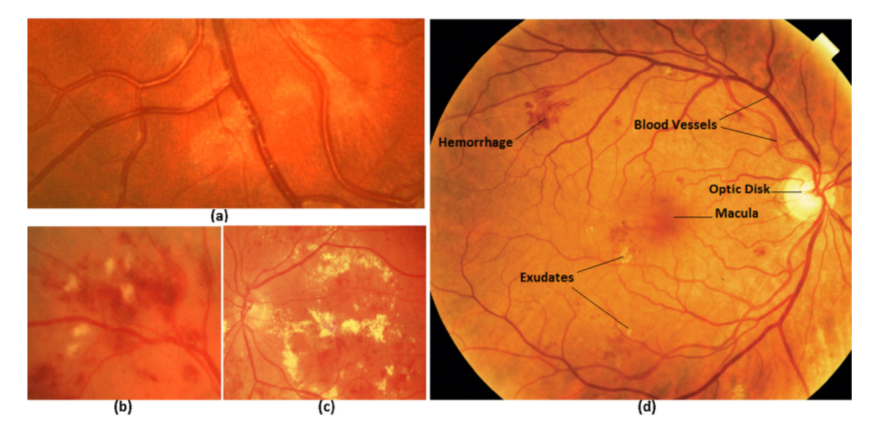
\includegraphics[width=1\textwidth]{Figures/image_ojo}
	\caption[Imagenes de Fondo de ojo]{Morfolog\'ia de im\'agenes de la retina: (a)Reflejo en el vaso central y fondo desigual, (b) Manchas algodonosas, (c)Exudados, (d) Estructura anat\'omica de la retina.}
	\label{fig:Fondo_de_ojo}
	}
\end{figure}	


Los m\'etodos de segmentaci\'on de los vasos de la retina son evaluados en tres bases de datos, DRIVE, HRF y ARIA.

DRIVE es una base de datos a disposici\'on del p\'ublico, que consta de un total de 40 im\'agenes a color con lesiones. Las fotograf\'ias se obtuvieron a partir de un programa de cribado de la retinopat\'ia diab\'etica en los Pa\'ises Bajos.
La poblaci\'on de selecci\'on consisti\'o en 453 sujetos de entre 31 y 86 a\~nos de edad. Cada imagen se ha comprimido JPEG , que es pr\'actica com\'un en los programas de cribado.\\
De las 40 im\'agenes en la base de datos, 7 contienen la patolog\'ia, es decir, los exudados, hemorragias y cambios del epitelio pigmentario. Ver (\ref{fig:Drive_images_retinal}) para un ejemplo de una imagen patol\'ogica y  una normal. Las im\'agenes fueron adquiridas mediante una camara no midri\'atica.\\

\begin{figure}[H]
	{
	\centering
	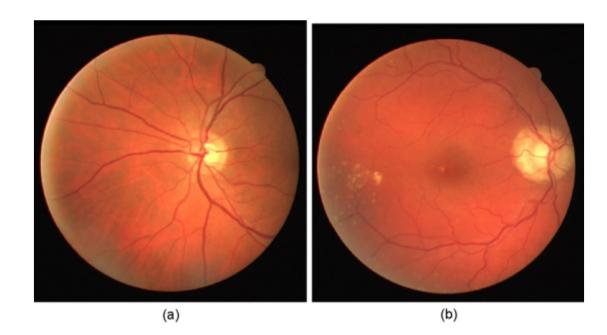
\includegraphics[width=1\textwidth]{Figures/Drive_images_retinal}
	\caption[Drive]{Im\'agen de la retina - DRIVE: (a) Retina saludable, (b) Retina con muestras patol\'ogicas.}
	\label{fig:Drive_images_retinal}
	}
\end{figure}	



En primer lugar, se determinaron los algoritmos a utilizar para mejorar el preprocesamiento de las im\'agenes, es decir, disminuir los efectos secundarios que se generan en la captura de im\'agenes de fondo de ojo como los nombrados anteriormente. 

Para la eliminaci\'on o extracci\'on del ruido se tuvieron en cuenta dos algoritmos: filtro de Difusi\'on Anisotr\'opica y filtro de  Coherencia.\\

En la actualidad existe una  amplia gama de metodologías para la detección automática de defectos  con  bajo contraste, todas ellas dependen de la buena adquisici\'on de la imagen, las condiciones de iluminaci\'on, el tipo de material que se desea inspeccionar, entre otros. A esto se le suma las características de los defectos que se quieran detectar, un ejemplo de estas características es el contraste que generan los defectos con respecto al fondo de la muestra, defectos que generan un mayor contraste son más fáciles de detectar que aquellos cuyo 
contraste es muy bajo.\\
Los defectos de bajo contraste se pueden clasificar dentro de dos clases con características diferentes para las etapas posteriores del proceso como la segmentación y clasificación. En la primera clase se encuentran los defectos oscuros de bajo contraste, estos se caracterizan por tener un nivel de gris más bajo. La segunda clase está conformada por defectos claros con bajo contraste, los cuales tienen un nivel de gris más alto 
en comparación al fondo en el que se encuentran embebidos. Se debe tener en cuenta que los defectos tienen niveles de gris diferentes (mayor o menor) al del resto del objeto de estudio, y  que el bajo contraste del defecto con respecto al  fondo del objeto  hace que la tarea de detección sea compleja tanto para las personas como para los sistemas de inspección industrial basados en visión por computador.\\

Esta secci\'on se centra en la evaluaci\'on del filtro de difusión anisotrópico como estrategia de realzado previa a la segmentación de defectos oscuros de bajo contraste en objetos pequeños de alta reflectividad con iluminación no homogénea.

Definici\'on del modelo de difusi\'on anisotr\'opico\\

La difusión anisotrópica propuesta por Perona y Malik \cite{perona1990scale} está dada de la siguiente manera: 

\begin{displaymath}
I_t=div\lbrack c_t(x,y)\nabla I_t(x,y)\rbrack  \hspace{2cm}(1)
\end{displaymath}

Donde div  es el operador de divergencia, \begin{displaymath}  \Delta \end{displaymath} es el operador Laplaciano y \begin{displaymath}
\nabla \end{displaymath}   es el operador gradiente.  \begin{displaymath} c_t(x,y)\end{displaymath} es el coeficiente 
de difusión definido en función del gradiente de tal forma que se adapte para que los bordes entre regiones sean preservados 
y los detalles intraregiones sean suavizados, \begin{displaymath} c_t(x,y)\end{displaymath} se define como se muestra a continuación:

\begin{displaymath}
c_t(x,y)=g(\nabla I_t(x,y))=1/\lbrack1+(\left|\nabla I_t/k\right|)^2\rbrack \hspace{2cm}(2)
\end{displaymath}

La difusión anisotrópica  se puede expresar de forma discreta de la siguiente manera:

\begin{displaymath}
I_{t+1}(x,y)=I_t(x,y) + \frac14{{{\sum_{i=1}^{4} \lbrack c_t^i(x,y).\nabla I_t^i(x,y)\rbrack}}} \hspace{2cm}(3)
\end{displaymath}

En el modelo discreto \begin{displaymath} \nabla I_t^i(x,y), i= 1,2,3,...,4 \end{displaymath} son los gradientes de los vecindarios en diferentes direcciones y \begin{displaymath} c_t^i(x,y) \end{displaymath} es el coeficiente de difusi\'on mencionado en (2), en esta ecuaci\'on k es una constante que se debe fijar de acuerdo a la aplicaci\'on del filtro seg\'un el desempe\~no que se busque.\\

El filtro de Difusi\'on anisotr\'opica es una técnica destinada a reducir el ruido de una imagen sin necesidad de retirar las piezas importantes del contenido de la imagen, por lo general los bordes, líneas u otros detalles que son importantes para la interpretación de la imagen, el modelo de difusión anisotrópico asemeja el proceso que crea un espacio de escala, donde una imagen genera una familia parametrizada de forma sucesiva cada vez más borrosas de imágenes, basadas en un proceso de difusión.\\ 

EXPLICAR UN POCO MAS DIFUSION ANISOTROPICA

El filtro de Coherencia ...This function COHERENCEFILTER will perform Anisotropic Diffusion of a 2D gray/color image or 3D image volume, Which will reduce the noise in an image while preserving the region edges, and will smooth along
the image edges removing gaps due to noise.\\ HACERLO COMPLETO 



Para la eliminaci\'on o extracci\'on del fondo se tuvieron en cuenta tres filtros denominados de paso bajo, el filtro de mediana, el filtro de media y el filtro gaussiano. 

El proceso de filtrado consiste en la aplicación a cada uno de los pixels de la imagen de una matriz de filtrado de tamaño N x N (generalmente de 3x3 aunque puede ser mayor) compuesta por números enteros y que genera un nuevo valor mediante una función del valor original y los de los pixels circundantes. El resultado final se divide entre un escalar, generalmente la suma de los coeficientes de ponderación. Los filtros se pueden expresar mediante una ecuación (6.1)

\begin{displaymath}
ND'_{i,j}=\frac{ND_{i-1,j-1}+ND_{i,\;j-1}+ND_{i+1,j-1}+ND_{i-1,j}+ND_{i,j}+ND_{i+1,j}+ND_{i-1,j+1}+ND_{i-1,j+1}ND_{i-1,j+1}}9 \hspace{2cm}(6.1)
\end{displaymath}

donde i y j representan la fila y la columna de cada pixel,  \[ND_{i;j}\] su Nivel Digital y \[ND'_{i,j}\] el Nivel Digital obtenido tras hacer el filtrado.\\

El objetivo de estos consiste en suavizar la im\'agen, son útiles cuando se supone que la imagen tiene gran cantidad de ruido y se quiere eliminar. También pueden utilizarse para resaltar la información correspondiente a una determinada escala (tamaño de la matriz de filtrado); 


\begin{itemize}
	\item[$*$] Filtro de la media, asigna al pixel central la media de todos los pixeles incluidos en la ventana. La matriz de filtrado estaría compuesta por unos y el divisor sería el número total de elementos en la matriz.
	
\begin{displaymath}
\begin{array}{l}\begin{array}{cccc}20&23&30&31\\22&21&29&30\\23&24&32&33\\29&31&34&37\end{array}\rightarrow\begin{array}{ccc}1&1&1\\1&1&1\\1&1&1\end{array}\rightarrow\begin{array}{cccc}N&N&N&N\\N&24.8&28.1&N\\N&27.2&30.1&N\\N&N&N&N\end{array}\\\\\;\;\;\;\;\;\;\;\;\;\;\;\;\;\;\;\;\;\;\;\;\;\;\;\;\;\;\;\text{Filtro de Media}\end{array}
\end{displaymath}
				
	\item[$*$] Filtro de la mediana tiene la ventaja de que el valor final del pixel es un valor real presente en la imagen y no un promedio, de este modo se reduce el efecto borroso que tienen las imagenes que han sufrido un filtro de media. Además el filtro de la mediana es menos sensible a valores exremos. El incoveniente es que resulta más complejo de calcular ya que hay que ordenar los diferentes valores que aparecen en los pixeles incluidos en la ventana y determinar cual es el valor central.
\begin{displaymath}
\begin{array}{l}\begin{array}{cccc}20&23&30&31\\22&21&29&30\\23&24&32&33\\29&31&34&37\end{array}\rightarrow\begin{array}{cccc}N&N&N&N\\N&23&30&N\\N&29&31&N\\N&N&N&N\end{array}\\\\\;\;\;\;\;\;\;\;\;\;\;\;\;\;\;\;\;\;\text{Filtro de Mediana}\end{array}
\end{displaymath}

	\item[$*$]Filtros gaussianos. Simulan una distribución gaussiana bivariante. El valor máximo aparece en el pixel central y disminuye hacia los extremos tanto más rápido cuanto menor sea el parámetro de desviación típica s. El resultado será un conjunto de valores entre 0 y 1. Para transformar la matriz a una matriz de números enteros se divide toda la matriz por el menor de los valores obtenidos. La ecuación para calcularla es:
	
	\begin{displaymath}
	g(x,y)=e^{-\frac{x^2+y^2}{2\ast s^2}} \hspace{2cm}(6.2)
	\end{displaymath}
	
	\begin{displaymath}
		G(x,y)=\frac{g(x,y)}{min_{x,y}(g(x,y))} \hspace{2cm}(6.3)
	\end{displaymath}
\end{itemize}


Para mejorar el contraste de las im\'agenes se utiliz\'o la t\'ecnica Contrast Limited AHE (CLAHE), la cual mejora el contraste  de la im\'agen en escala de grises mediante la transformaci\'on de los valores. CLAHE opera sobre peque\'nas regiones de la im\'agen , llamados azulejos , en lugar de toda la im\'agen.El contraste de cada regi\'on es mayor, por lo que el histograma de la zona de salida coincide aproximadamente con el histograma especificado por el parámetro ' Distribución ' . Los azulejos vecinos se combinan a continuación, utilizando la interpolación bilineal para eliminar los límites inducidas artificialmente . El contraste , sobre todo en áreas homogéneas , puede ser limitada para evitar la amplificación de cualquier ruido que pudiera estar presente en la imagen.


Con los métodos de filtrado definidos y analizados teniendo en cuenta sus ventajas y desventajas, se realizaron cuatro pipelines para determinar cu\'al de estos es el mejor para utilizar en los sets de im\'agenes propuestos.

\begin{itemize}
	    \item Pipeline 1 -> Extracci\'on de fondo(Mediana, Media o Gaussiano)  +  Realce(CLAHE)  +  Extracci\'on de ruido(Filtro anisotr\'opico o Filtro de Coherencia)
		\item Pipeline 2 -> Realce(CLAHE) +  Extracci\'on de ruido(Filtro anisotr\'opico o Filtro de Coherencia)
		\item Pipeline 3 -> Realce(CLAHE) +  Extracci\'on de fondo(Mediana, Media o Gaussiano)
		\item Pipeline 4 -> Realce(CLAHE)  + Extracci\'on de fondo(Mediana, Media o Gaussiano)   +  Extracci\'on de ruido(Filtro anisotr\'opico o Filtro de Coherencia)
\end{itemize}






%-----------------------------------
%	SECTION 3
%-----------------------------------

\section{Extracci\'on de caracter\'isticas}


%----------------------------------------------------------------------------------------
%	SECTION 4
%----------------------------------------------------------------------------------------

\section{M\'etodo de segmentaci\'on}


% Chapter Template

\chapter{Resultados} % Main chapter title

En este cap\'itulo  describiremos los datos utilizados en 	nuestros experimentos, las m\'etricas de calidad utilizadas para evaluar los resultados, la manera en la que se  utilizaron los datos y los resultados obtenidos.\\

En la secci\'on  4.1 se describen los materiales utilizados para la realizaci\'on de este trabajo final. Los tipos de dataset utilizados con las caracter\'isticas correspondientes a cada tipo de im\'agenes, dispositivos de captura, resoluci\'on de las im\'agenes, entre otras.\\

En la secci\'on 4.2  se estudian las m\'etricas de calidad utilizadas..\\

En la secci\'on 4.3 se exponen los resultados obtenidos durante el dise\'no del algoritmo..\\

En la secci\'on 4.3.1 se exponen y analizan los resultados obtenidos durante la etapa de preprocesamiento. \\

En la secci\'on 4.3.2 ..\\

En la secci\'on 4.3.3 ..\\

En la secci\'on 4.4 ..\\

En la secci\'on 4.5 ..\\



\label{Chapter4} % Change X to a consecutive number; for referencing this chapter elsewhere, use \ref{ChapterX}

%----------------------------------------------------------------------------------------
%	SECTION 1
%----------------------------------------------------------------------------------------

\section{Materiales}

Hacer mañana
%-----------------------------------
%	SECTION 2
%-----------------------------------
\section{M\'etricas de calidad utilizadas}


%-----------------------------------
%	SECTION 3
%-----------------------------------

\section{Resultados obtenidos durante el dise\'no del algoritmo}

%----------------------------------------------------------------------------------------
%	SECTION 4
%----------------------------------------------------------------------------------------

\subsection{Preprocesamiento}

%----------------------------------------------------------------------------------------
%	SUBSECTION 5
%----------------------------------------------------------------------------------------

\subsection{Extracci\'on de caracter\'isticas}


%----------------------------------------------------------------------------------------
%	SECTION 5
%----------------------------------------------------------------------------------------

\subsection{Entrenamiento y clasificaci\'on}

\section{Resultado del algoritmo de segmentaci\'on propuesto}

\section{Discusi\'on}

 
% Chapter Template

\chapter{Conclusiones} % Main chapter title

\label{Chapter5} % Change X to a consecutive number; for referencing this chapter elsewhere, use \ref{ChapterX}

%----------------------------------------------------------------------------------------
%	SECTION 1
%----------------------------------------------------------------------------------------

\section{Main Section 1}

 

%----------------------------------------------------------------------------------------
%	THESIS CONTENT - APPENDICES
%----------------------------------------------------------------------------------------

\appendix % Cue to tell LaTeX that the following "chapters" are Appendices

% Include the appendices of the thesis as separate files from the Appendices folder
% Uncomment the lines as you write the Appendices

% Appendix A

\chapter{Appendix Title Here} % Main appendix title

\label{AppendixA} % For referencing this appendix elsewhere, use \ref{AppendixA}

Write your Appendix content here.
%\input{Appendices/AppendixB}
%\input{Appendices/AppendixC}

%----------------------------------------------------------------------------------------
%	BIBLIOGRAPHY
%----------------------------------------------------------------------------------------

\printbibliography[heading=bibintoc]

%----------------------------------------------------------------------------------------

\end{document}  
